\documentclass[12pt, a4paper]{article}
\usepackage[utf8]{inputenc}
\usepackage[spanish]{babel}
\usepackage{mathtools}
\usepackage{graphicx}
\graphicspath{ {./images/} }
\usepackage{blindtext}
\usepackage{enumitem}
\providecommand{\abs}[1]{\lvert#1\rvert}

\usepackage[ruled,vlined ]{algorithm2e}
\usepackage{algorithmic}

\usepackage{lscape}

\usepackage{geometry}
 \geometry{
 a4paper,
 total={160mm,245mm},
 left=25mm,
 top=30mm,
 }
 
 \usepackage[backend=biber,sorting=none]{biblatex}
\bibliography{referencias}



\title{CORDIC}
\author{Juan Carlos Llamas Núñez }
\date{Abril 2021}

\begin{document}

\maketitle
\section{Introducción}
\setlength{\parskip}{1em}
CORDIC es un algoritmo para el cálculo de funciones trigonométricas e hiperbólicas. Toma su nombre del inglés (COordinate Rotation DIgital Computer) y también es conocido como el método dígito a dígito o el algoritmo de Volder. Tiene su origen en 1956, cuando Jack E. Volder~\cite{volder}, que trabajaba en el departamento de electrónica de la empresa de aviación Convair, buscaba remplazar un resolver\footnote{Un resolver es un dispositivo electromecánico que convierte el movimiento mecánico en una señal electrónica analógica.} analógico en la computadora de uno de sus aviones bombarderos. La finalidad era mejorar el rendimiento y la precisión de las operaciones que se realizaban. En su investigación, Volder hizo uso de la siguiente fórmula publicada en \textit{CRC Handbook of Chemestry and Physics}:


Si $tan(\varphi)=2^{-n}$ y definimos $K_n=\sqrt{1+2^{-2n}}$ entonces 
\[
K_nsin(\theta \pm \varphi)=sin(\theta) \pm 2^{-n} cos(\theta)
\]\[
K_ncos(\theta \pm \varphi)=sin(\theta) \mp 2^{-n} cos(\theta)
\]

Este resultado se obtiene fácilmente aplicando las identidades del seno suma\footnote{$sin(\alpha + \beta)=sin(\alpha)cos(\beta) + cos(\alpha)sin(\beta)$} y coseno suma\footnote{$cos(\alpha + \beta)=cos(\alpha)cos(\beta) - sin(\alpha)sin(\beta)$} y la relación $\frac{1}{cos^2(\alpha)}=1+tan^2\alpha$.

Las técnicas empleadas por Volder fueron similares a otras publicadas por Henry Briggs algo más de tres siglos antes (1624) o por Robert Flower en 1771. Sin embargo, su principal aportación fue una implementación optimizada para máquinas de estados finitos de baja complejidad.
\section{Conceptos previos}
Antes de comenzar a explicar el algoritmo, conviene recordar algunos conceptos relacionados con las rotaciones en el plano. Si consideramos la circunferencia de centro $(0,0)$ y radio 1, las coordenadas cartesianas $(x,y)$ de todos sus puntos $P$ cumplen la ecuación $x^2+y^2=1$. Esos puntos se pueden representar en coordenadas polares como $P=(1,\theta)$  donde $\theta$ es el ángulo\footnote{Los ángulos los vamos a medir siempre en radianes salvo mención expresa de lo contrario.} entre la recta definida por unir el punto $P$ con el origen y el eje de abscisas, y 1 es el radio. Si expresamos el punto en coordenadas cartesianas en función del ángulo tenemos que $P=(cos(\theta),sin(\theta))$. Si queremos mandar el punto P a otro punto Q de la circunferencia, lo podemos hacer mediante una rotación, es decir, al punto $P=(cos(\theta),sin(\theta))$ enviarlo a $Q=(cos(\theta+\omega),sin(\theta+\omega))$. Por las fórmulas del seno suma y coseno suma, esto se puede expresar de forma matricial como:
\[
\begin{pmatrix*}[r]
  cos(\omega) & -sin(\omega)\\
  sin(\omega) & cos(\omega) 
 \end{pmatrix*}
\begin{pmatrix*}[r]
  cos(\theta)\\
  sin(\theta)
 \end{pmatrix*}
 =
 \begin{pmatrix*}[r]
  cos(\theta+\omega)\\
  sin(\theta+\omega)
 \end{pmatrix*}.
\]
Es decir, podemos codificar una rotación como la aplicación de una función lineal a un vector, que consiste en multiplicarlo por una matriz $R_\omega$ por la izquierda. Sacando el coseno fuera podemos descomponer la matriz $R_\omega$ como
\[
R_\omega = 
\begin{pmatrix*}[r]
  cos(\omega) & -sin(\omega)\\
  sin(\omega) & cos(\omega) 
 \end{pmatrix*}
= cos(\omega)
\begin{pmatrix*}
  1 & -tan(\omega)\\
  tan(\omega) & 1 
 \end{pmatrix*}
 =
 \]
 \[
 \frac{1}{\sqrt{1+tan^2(\omega)}}
 \begin{pmatrix*}
  1 & -tan(\omega)\\
  tan(\omega) & 1 
 \end{pmatrix*}
\]
\section{Modos de operación}
El algoritmo CORDIC cuenta con dos modos de operación que nos permiten calcular los valores de la gran mayoría de funciones trigonométricas.
\subsection{Modo \textit{rotación}}
El objetivo de este modo es calcular el seno y el coseno de un determinado ángulo $\theta$ dado. El algoritmo es iterativo y en cada paso construye un vector de módulo 1 (que se puede identificar con un punto de la circunferencia goniométrica). Cada nuevo vector va a ser el resultado de rotar el vector construido en la iteración anterior, en sentido horario o antihorario, un ángulo de amplitud $\omega_i$. Estos ángulos van a ser elegidos de manera específica para que, como vamos a ver, las operaciones a realizar se simplifiquen lo máximo posible. Comenzaremos con $v_0 =\begin{pmatrix*}
  1\\
  0
 \end{pmatrix*}$ y $v_{i+1}$ se calcula a partir de $v_i$ como
 \[
 v_{i+1}=R_{\omega_i} v_i=
  \frac{1}{\sqrt{1+tan^2(\omega_i)}}
 \begin{pmatrix*}
  1 & -tan(\omega_i)\\
  tan(\omega_i) & 1 
 \end{pmatrix*}v_{i}
 =
  \]
  \[
  \frac{1}{\sqrt{1+2^{-2i}}}
   \begin{pmatrix*}
  1 & -\delta_i2^{-i}\\
  \delta_i2^{-i} & 1 
 \end{pmatrix*}v_{i}
=
 K_i\begin{pmatrix*}
  1 & -\delta_i2^{-i}\\
  \delta_i2^{-i} & 1 
 \end{pmatrix*}v_{i}
 \]
 donde $K_i=\frac{1}{\sqrt{1+2^{-2i}}}$, $\delta_i$ es $+1$ o $-1$, según el ángulo de rotación sea positivo o negativo, y hemos particularizado para los ángulos $\omega_i\in(-\pi/2,\pi/2)$ con módulo $\abs{\omega_i}=arctan(2^{-i})$, es decir, $tan(\abs{\omega_i})=2^{-i}$.
 
 
 Para determinar el valor de $\delta_i$ necesitamos almacenar de alguna manera el ángulo asociado al vector $v_{i}$. Como la composición de rotaciones es una rotación de ángulo suma, es decir, $R_\alpha R_\beta=R_{\alpha+\beta}$, se sigue que hacer una serie de rotaciones de ángulo $\omega_i$ con $i = 0, 1,\ldots n$ equivale a hacer una única rotación de ángulo $\phi_n=\sum_{i=0}^n \omega_i$. Por tanto, decidir si la rotación se hace en sentido horario o antihorario consiste en comprobar si $\phi_i$ es mayor o menor que $\theta$, o equivalentemente, si $\theta-\phi_i$ es menor o mayor que 0. Se puede expresar esto de manera explícita con las recurrencias:
 \[
 z_0=\theta,\;\;\;\; z_{i+1}=z_{i}-\delta_iarctan(2^{-i}),\;\;\;\;
 \delta_i=\begin{cases}
+1,&\mathrm{ si }\quad z_{i}\geq 0\\
-1,&\mathrm{ si }\quad z_{i}<0
\end{cases}.
 \]
 De esta forma $z_i$ almacena la diferencia entre el ángulo del que queremos calcular su seno y coseno y el ángulo asociado al vector $v_i$. Nuestro objetivo es hacer tender $z_i$ a 0. Se podría pensar que $z_i$ es difícil de calcular porque involucra el cómputo de arcotangentes. Sin embargo, en la práctica se guardan en una lookup table (LUT) los valores de los ángulos que nos interesan, es decir, $arctan(2^{-i})$ para $i = 0, 1,\ldots n$. Si estos valores, que son siempre los mismos, ya los tenemos precalculados, lo único que tenemos que hacer es sumarlos o restarlos según corresponda. Además, cuando $x$ es suficientemente pequeño podemos aproximar $arctan(x)$ por $x$, lo que, traducido a nuestro problema, supone que si $i$ es suficientemente grande $arctan(2^{-i})\approx2^{-i}$. Esto implica que, en la práctica, es suficiente con guardar en la LUT solamente ``unos pocos'' ángulos.
 
 Por tanto, si realizamos $n$ iteraciones del algoritmo se tiene que 
 \[
 v_n=\left(\prod_{i=0}^{n-1}R_{\omega_i} \right) v_{0}=\prod_{i=0}^{n-1}\begin{pmatrix*}
  1 & -\delta_i2^{-i}\\
  \delta_i2^{-i} & 1 
 \end{pmatrix*}\left[\left(\prod_{i=0}^{n-1}K_i\right) v_{0}\right],
 \]
 donde hemos sacado todas las $K_i$ fuera porque son escalares. Ahora llamamos $K(n)=\prod_{i=0}^{n-1}K_i$ y $M_n$ a la matriz 2x2 resultante de hacer el producto de las matrices. Como el número de iteraciones a realizar es conocido de antemano, podemos inicializar el algoritmo, en lugar de con $v_0$, con $\hat{v}_0 = K(n)v_0=\begin{pmatrix*}
  K(n)\\
  0
 \end{pmatrix*}$. Como hacíamos con los ángulos, estos valores de $K(n)$ pueden estar precalculados para cada $n$ y guardados en una LUT. También se suele almacenar el valor $K=\lim_{n \to \infty}K(n)\approx0.6072529250088812561694$ para valores de $n$ suficientemente grandes luego, nuevamente, solo tenemos que guardar ``unos pocos'' valores de $K(n)$. Otras versiones del algoritmo renuncian a la multiplicación de $v_0$ por $K$ y recuerdan que el resultado aparece multiplicado por un factor de escala $A=\frac{1}{K}\approx 1.6467602025812107$. La interpretación geométrica de esta versión es que hacemos rotaciones y homotecias, luego los vectores dejan de tener módulo 1, pero conservan el ángulo, que es lo que verdaderamente nos interesa.
 
 Nos queda todavía multiplicar $M_n$ por $v_0$, lo cual se hace asociando por la derecha, multiplicando matriz por vector iterativamente. Estas operaciones son todas multiplicaciones de la forma 
 \[
 \begin{pmatrix*}
  x_{i+1}\\
  y_{i+1}
 \end{pmatrix*}=
 \begin{pmatrix*}
  1 & -\delta_i2^{-i}\\
  \delta_i2^{-i} & 1 
 \end{pmatrix*}
 \begin{pmatrix*}
  x_i\\
  y_i
 \end{pmatrix*}
 =\begin{pmatrix*}
  x_i -\delta_i2^{-i}y_i\\
  y_i +\delta_i2^{-i}x_i
 \end{pmatrix*}.
 \] Aquí se puede apreciar el gran poder de este algoritmo: las operaciones a realizar son sumas, restas y divisiones entre potencias de 2, que no es otra cosa que un desplazamiento de bits. No hace falta efectuar ningún tipo de multiplicación que requiera un módulo multiplicador externo.
 
 La ejecución de este algoritmo nos lleva al resultado deseado. Según aumenta $i$, el ángulo de la composición de las rotaciones se acerca cada vez más a $\theta$ o, alternativamente, $z_i$ tiende a 0. Por construcción, en cada iteración nos aproximamos más a 0 (en valor absoluto) ya que decidimos rotar en sentido horario o antihorario según $\theta-\phi_i$ sea mayor o menor que 0, respectivamente. Por tanto, el resultado final es un vector $v_n=\begin{pmatrix*}
  x_n\\
  y_n
 \end{pmatrix*}$ de módulo 1 y de ángulo en coordenadas polares $\sum_{i=0}^{n-1} \omega_i\approx \theta$, luego sus componentes serán $x_n=cos(\sum_{i=0}^{n-1} \omega_i)\approx cos(\theta)$ e $y_n=sin(\sum_{i=0}^{n-1} \omega_i)\approx sin(\theta)$.
 \subsection{Modo \textit{vectorización}}
 En este modo alternativo, el $input$ no es un ángulo, sino un vector, no necesariamente unitario, en el primer o el cuarto cuadrante, es decir, con primera coordenada positiva. El objetivo va a ser realizar rotaciones, de manera análoga a como se hacían en el modo \textit{rotación}, para llevar el vector al eje X, es decir, haciendo tender a 0 el valor $y_i$ según aumenta $i$. Si esta vez inicializamos el valor de $z_0$ a 0, obtendremos que $z_i$ almacena el valor de las rotaciones que vayamos efectuando. Para decidir en que sentido rotar, en esta ocasión nos fijamos en el signo de $y_i$ y las recurrencias quedan como:
 \[
 v_0=\begin{pmatrix*}
  x_0\\
  y_0
 \end{pmatrix*}, \;\;\;
 z_0=0,\;\;\;z_{i+1}=z_{i}-\delta_i arctan(2^{-i}),\;\;\;
 \delta_i=\begin{cases}
+1,&\mathrm{si}\quad y_{i}\leq0\\
-1,&\mathrm{si}\quad y_{i}>0
\end{cases}
 \]
 y $v_i$ calculado como antes, con la salvedad de que no hace falta multiplicar en ningún momento por los $K_i$.
 Para un valor de $n$ suficientemente grande se tiene que $y_n\approx0$, $z_n\approx arctan(\frac{y_0}{x_0})$ y $x_n = \frac{1}{K(n)}\sqrt{x_0^2+y_0^2}$.
 
 Nótese que el cálculo de $x_{i+1}$, $y_{i+1}$ y $z_{i+1}$ no cambia respecto al modo rotación. La única diferencia es la manera de calcular el sentido del giro, es decir $\delta_i$, y los valores iniciales del algoritmo $x_0$, $y_0$ y $z_0$.
 \section{Aplicaciones}
 Los dos modos de funcionamiento anteriormente descritos nos presentan las siguientes posibilidades de cálculo:
 \begin{enumerate}
    \item \textbf{Senos y cosenos.}
    Para calcular el seno o el coseno de un ángulo $\theta$ dado basta aplicar el modo de operación \textit{rotación} ($n$ iteraciones, $x_0=K(n)$, $y_0=0$, $z_0=\theta$). El valor obtenido en $x_n$ será el coseno y en $y_n$ aparecerá el seno. Nótese que se calcula simultáneamente el seno y el coseno, lo cual puede suponer una mejora en rendimiento.
    \item \textbf{Cambio de coordenadas.}
    Podemos pasar de coordenadas polares a cartesianas y viceversa. Para pasar de coordenadas polares a cartesianas se tiene que si $P=(r,\theta)$ en polares, entonces $P=(rcos(\theta), rsin(\theta))$ en coordenadas cartesianas. Basta entonces aplicar el modo \textit{rotación} ($n$ iteraciones, $x_0=rK(n)$, $y_0=0$, $z_0=\theta$) para obtener $x_n\approx rcos(\theta)$, $y_n\approx rsin(\theta)$.
 Para pasar de coordenadas cartesianas $(x,y)$ a polares podemos utilizar el modo \textit{vectorización} ($n$ iteraciones, $x_0=x$, $y_0=y$, $z_0=0$). Entonces en $z_n$ obtendremos el ángulo y en $x_n$ tendremos $r$ multiplicado por el factor de escalado $\frac{1}{K(n)}$. Multiplicar el resultado por $K(n)$ va en contra de la filosofía de este algoritmo, que intenta simplificar al máximo las operaciones de multiplicación con el objetivo de no usar módulos multiplicadores externos. Sin embargo, en este caso es necesario. Aun así, solo necesitamos una multiplicación, por lo que la mejora puede ser considerable. También hay que hacer notar que el vector introducido en el modo \textit{vectorización} ha de tener la primera componente positiva, lo cual no supone ninguna restricción en la práctica porque el cálculo de las razones trigonométricas puede reducirse a ángulos del primer cuadrante simplemente cambiando algunos signos de manera apropiada.
   \item \textbf{Arcotangentes y módulo de vectores.}
   El cálculo de la arcotangente de un valor $y$ se deduce inmediatamente de la aplicación del modo \textit{vectorización} ($n$ iteraciones, $x_0=1$, $y_0=y$, $z_0=0$). El resultado se obtiene en $z_n$. Para el módulo, basta recurrir a lo que hacíamos en el cambio de coordenadas cartesianas a polares.
\end{enumerate}
 \section{Generalizaciones}
En 1971, John Stephen Walther~\cite{10.1145/1478786.1478840}\cite{10.5555/352135.2812970}, de  Hewlett-Packard (HP), propuso una generalización del algoritmo CORDIC que fue implementada en la calculadora HP-35, la primera calculadora de bolsillo fabricada por la empresa y primera calculadora científica de bolsillo del mundo con funciones trigonométricas, logarítmicas y exponenciales. Introdujo dos parámetros $f(x)$ y $m$ que permitieran un mayor rango de cálculos. Las ecuaciones recursivas quedan:
\[
\begin{cases}
x_{i+1}=x_{i}-m\delta_{i}2^{-i}y_i\\
y_{i+1}=y_{i}+\delta_{i}2^{-i}x_i\\
z_{i+1}=z_{i}-\delta_{i}f(2^{-i})
\end{cases}.
\]
Nos damos cuenta de que si $m=1$ y $f(x)=arctan(x)$, las ecuaciones resultan ser:
\[
\begin{cases}
x_{i+1}=x_{i}-\delta_{i}2^{-i}y_i\\
y_{i+1}=y_{i}+\delta_{i}2^{-i}x_i\\
z_{i+1}=z_{i}-\delta_{i}arctan(2^{-i})
\end{cases},
\]
es decir, las mismas que para el CORDIC básico.
Estudiamos los casos en los que $m=0$ y $f(x)=x$ (Rotación Lineal) y $m=-1$ y $f(x)=arctanh(x)$ (Rotación Hiperbólica).
 \subsection{Rotación Lineal}
 En este caso, las ecuaciones quedan:
 \[
\begin{cases}
x_{i+1}=x_{i}\\
y_{i+1}=y_{i}+\delta_{i}2^{-i}x_i\\
z_{i+1}=z_{i}-\delta_{i}2^{-i}
\end{cases}.
\]
Para el modo \textit{rotación}, en el que el sentido de giro era determinado como \[ \delta_i=\begin{cases}
+1,&\mathrm{ si }\quad z_{i}\geq0\\
-1,&\mathrm{ si }\quad z_{i}<0
\end{cases}\] para hacer tender $z_i$ a 0, entonces $x_n=x_0$, $z_n\approx 0$ y se puede probar por inducción que $y_n=y_0+(z_0-z_n)x_0\approx y_0+z_0x_0$. Tomando $y_0=0$, $x_0=a$ y $z_0=b$, tras un número suficientemente grande de iteraciones, obtenemos que $y_n\approx ab$. Análogamente, para el modo \textit{vectorización}, donde hacíamos tender $y_i$ a 0 eligiendo 
\[ \delta_i=\begin{cases}
+1,&\mathrm{ si }\quad y_{i}\leq0\\
-1,&\mathrm{ si }\quad y_{i}>0
\end{cases},\]podemos concluir que  $x_n=x_0$, $y_n\approx 0$ y $z_n=z_0+\frac{y_0-y_n}{x_0}\approx z_0+\frac{y_0}{x_0}$. Eligiendo $z_0=0$, $y_0=a$ y $x_0=b$, y para un número grande de iteraciones, obtenemos en $z_n$ un valor próximo a $a/b$.

Con esta generalización hemos conseguido calcular también multiplicaciones y divisiones sin la necesidad de añadir ningún módulo extra, más allá de incluir posibles multiplexores y/o señales de control en la ruta de datos. Seguimos utilizando únicamente sumas, restas y desplazamientos de bits.
 \subsection{Rotación Hiperbólica}
 En este caso, las ecuaciones quedan:
 \[
\begin{cases}
x_{i+1}=x_{i}+\delta_{i}2^{-i}y_i\\
y_{i+1}=y_{i}+\delta_{i}2^{-i}x_i\\
z_{i+1}=z_{i}-\delta_{i} arctanh(2^{-i})
\end{cases}.
\]
Para el modo \textit{rotación} se puede probar~\cite{10.1145/1478786.1478840} que
 \[
\begin{cases}
x_n=B_n(x_0cosh(z_0)+y_0sinh(z_0))\\
y_n=B_n(y_0cosh(z_0)+x_0sinh(z_0))\\
z_n\approx 0
\end{cases}
\textrm{, con } B_n =\prod_{i=0}^{n-1}\sqrt{1-2^{-2i}}
\]
y para el modo \textit{vectorización} se tiene que 
\[
\begin{cases}
x_n=B_n\sqrt{x_0^2 -y_0^2}\\
y_n\approx0\\
z_n= z_0+arctanh(\frac{y_0}{x_0})
\end{cases} \textrm{con } B_n \textrm{ definido como antes.}
\]
Con este nuevo modo y elecciones convenientes de los valores de entrada ($x_0$, $y_0$, $z_0$ y modo de operación) podemos calcular las funciones $cosh(x)$, $sinh(x)$ y $arctanh(x)$. Si también podemos combinar los modos de rotación básico, lineal e hiperbólico, podemos generar otras funciones usando igualdades conocidas como:
\[tan(x)=\frac{sin(x)}{cos(x)},\;\;\;\; cotan(x)=\frac{cos(x)}{sin(x)},\;\;\;\; tanh(x)=\frac{sinh(x)}{cosh(x)},\]
\[cotanh(x)=\frac{cosh(x)}{sinh(x)}, \;\;\;\;sec(x)=\frac{1}{cos(x)},\;\;\;\; cosec(x)=\frac{1}{sin(x)},\;\;\;\; \]
\[sech(x)=\frac{1}{cosh(x)},\;\;\;\; cosech(x)=\frac{1}{sinh(x)},\;\;\;\; exp(x)=sinh(x)+cosh(x),\]
\[ln(w)=2arctanh(y/x)\;\; \textrm{ con }\;\;x=w+1\;\;\textrm{ e }\;\;y=w-1\;\;\textrm{ o }\]
\[\sqrt{w}=\sqrt{x^2-y^2} \;\; \textrm{para}\;\; x=w+1/4 \;\;\textrm{ e }\;\; y=w-1/4 \textrm{ . }\]
No debemos olvidar que todo esto lo podemos conseguir simplemente con sumas, restas, desplazamientos y LUTs, necesarias para almacenar los valores de $arctanh(2^{-i})$ para $i = 0, 1,\ldots n$.\footnote{También se cumple que $arctanh(x)\approx x$ para $x$ pequeños.} No necesitamos añadir hardware adicional, salvo las modificaciones obvias en la ruta de datos y la unidad de control del sistema algorítmico para elegir el modo de funcionamiento, tipo de rotación y valores iniciales.

No es muy difícil imaginar que las aplicaciones de este algoritmo van más allá del cálculo de funciones trigonométricas, hiperbólicas, divisiones, productos y raíces cuadradas. Además, se pueden realizar multiplicaciones de números complejos y operaciones con matrices, como calcular soluciones a sistemas lineales, estimar valores propios, descomposición en valores singulares, factorización QR y muchas otras.
Algunos campos en los que es usado este algoritmo son el procesamiento de imágenes y señales, sistemas de comunicacción, robótica o diseño gráfico, además de la computación científica y técnica de propósito general. 
\section{Iteraciones, precisión y convergencia}
Una vez conocemos el funcionamiento del algoritmo es conveniente aclarar algunos asuntos que hemos ido dejando en el aire durante la explicación del funcionamiento del mismo. Hemos planteado los resultados de convergencia como ciertos para cualesquiera parámetros de entrada, lo cual no siempre es cierto, y no hemos concretado cómo de grande debe ser $n$ para obtener resultados suficientemente satisfactorios. En esta sección pretendemos despejar las dudas sobre estos aspectos técnicos.

En primer lugar, comenzamos hablando sobre convergencia. Es natural esperar de un algoritmo iterativo que, a medida que se hacen más iteraciones, el resultado obtenido se acerque más al resultado real. Sin embargo, advertimos que esto no siempre es así. Es por tanto conveniente establecer un rango de valores o dominio de los parámetros en el que se cumple esta propiedad. Así, asociada a cada uno de los modos de operación y tipos de CORDIC, tendremos unas restricciones en los parámetros. Muchas veces, estos rangos se pueden extender haciendo uso de identidades conocidas. En la práctica, los cálculos del seno, coseno, tangente y arcotangente no presentan ningún problema. Sin embargo, los cálculos relacionados con las funciones hiperbólicas, la exponencial, el logaritmo, la raiz cuadrada y productos y divisiones presentan un rango de valores más restrictivo y requieren del uso de fórmulas, en algunos casos complejas, para extender dichos rangos.

Alternativamente al uso de identidades para ampliar el rango de parámetros, los rusos Vladimir Baykov y Vladimir Smolov propusieron la realización de dobles iteraciones para los cálculos en los que intervinieran estas últimas funciones que resultaban más problemáticas~\cite{baykov1}. Al contrario que el método orginial del CORDIC, donde cada iteración se realiza una sola vez, con las iteraciones dobles se repetía cada iteración dos veces. Fueron aún más lejos~\cite{baykov2}, ya que probaron que para un sistema numérico de base arbitraria $B$ el número de repeticiones de cada iteración para las funciones:
\begin{itemize}
    \item seno, coseno y arcotangente debe ser $B-1$.
    \item logaritmo, exponencial, seno, coseno y arcotangente hiperbólicos debe ser $B$.
    \item arcoseno y arcocoseno debe ser $2B-2$.
    \item arcoseno y arcocoseno hiperbólicos debe ser $2B$.
\end{itemize}

Queda por saber que valores de $n$ nos garantizan una precisión suficientemente buena. En la práctica tomando $n=40$ se obtienen un resultado correcto hasta la décima cifra decimal (en base 10 y unas 30 en base 2). Otros experimentos empíricos \cite{tesis} nos arrojan que para valores de $n=16$ y $n=32$ las cifras decimales correctas son 3 y 7 (del orden de 10 y 20 en base 2), respectivamente, lo que concuerda con la idea que teníamos de que al aumentar $n$ aumentaba la precisión del resultado. Tras estas intuiciones sobre convergencia podemos comprender por qué este algoritmo recibe el nombre de método de dígito a dígito, ya que la convergencia se produce aproximadamente a razón de un bit por iteración.
\section{Implementación}
Para la implementación nos vamos a restringir al caso del CORDIC básico, ya que los demás casos no aportan nada nuevo, en el sentido de que la estructura del diseño sigue siendo la misma, y solo dificultan su comprensión. Presentamos el algoritmo del CORDIC, el diagrama ASM en la Figura \ref{fig:DASM}, el diagrama de transición de estados en la Figura \ref{fig:Dest}, la ruta de datos en la Figura \ref{fig:RdD} y la tabla de señales de control en la Figura \ref{fig:Tb}, siguiendo el estándar de diseño algorítmico.

\begin{algorithm}[h]
\SetAlgoLined
 $N\gets n$\;
 $X\gets x_0$\;
 $Y\gets y_0$\;
 $Z\gets z_0$\;
 $i\gets 0$\;
 $MODE\gets modeOper$\;
 \While{$i<N$}{
  \eIf{$MODE==1$}{
   $\delta_i\gets sign(Z)$\;
   }{
   $\delta_i\gets -sign(Y)$\;
  }
  $Z\gets Z+\delta_i arctan(2^{-i})$\;
  //Asignaciones simultáneas\;
  $X\gets X-(\delta_iY >>i)$\;
  $Y\gets Y+(\delta_iX >>i)$\;
  $i\gets i+1$\;
 }
 \caption{CORDIC}
\end{algorithm}

\clearpage

\begin{figure}[h]
      \centering
      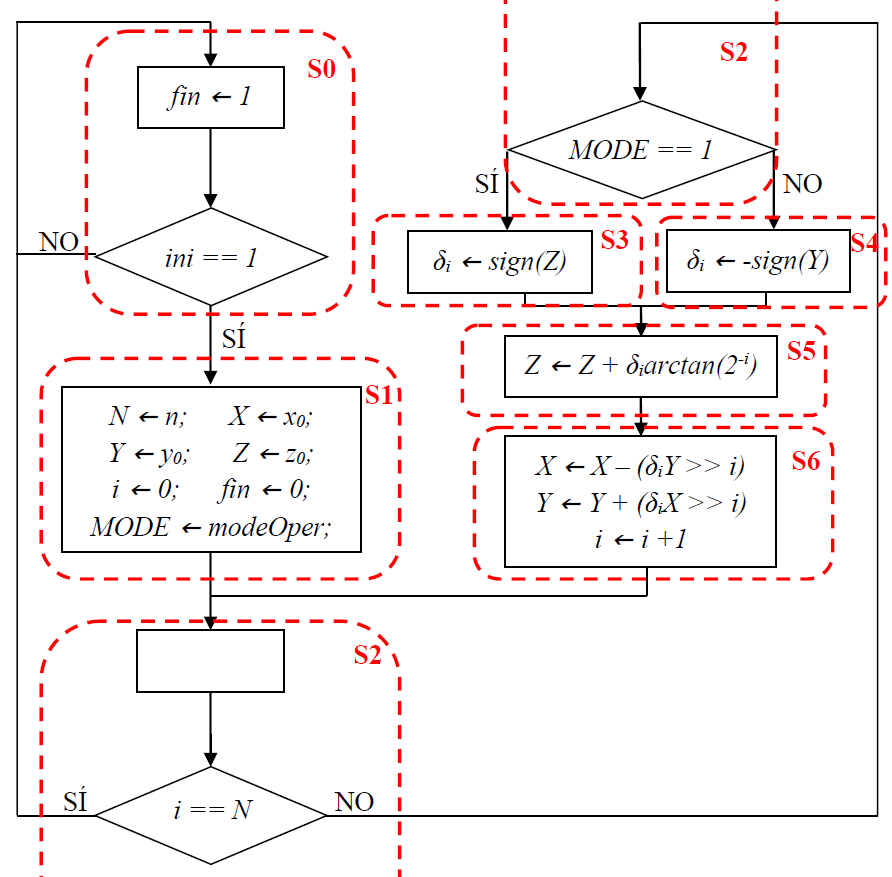
\includegraphics[scale=0.5]{images/Diagrama ASM.png}
      \caption {Diagrama ASM}
      \label{fig:DASM}
\end{figure}

\hfill
\break

\begin{figure}[h]
      \centering
      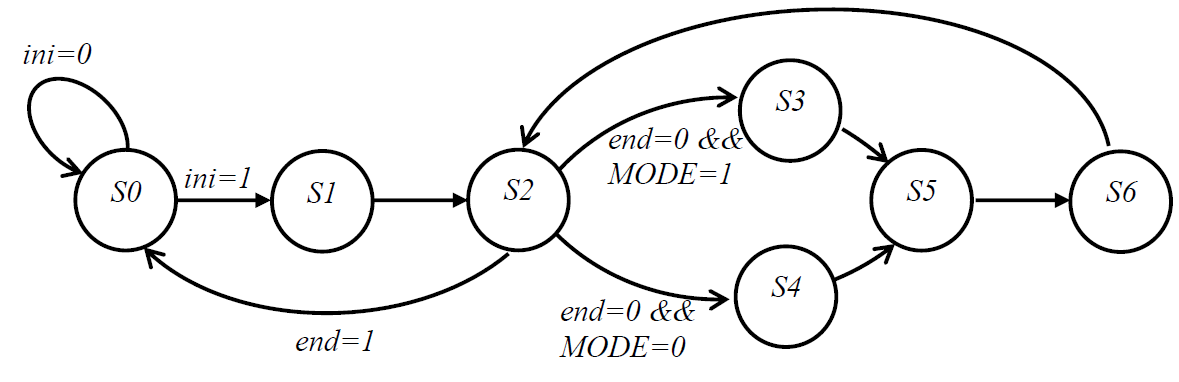
\includegraphics[scale=0.4]{images/Diagrama de estados.png}
      \caption {Diagrama de transición de estados}
      \label{fig:Dest}
\end{figure}

\begin{landscape}
\begin{figure}[h]
      \centering
      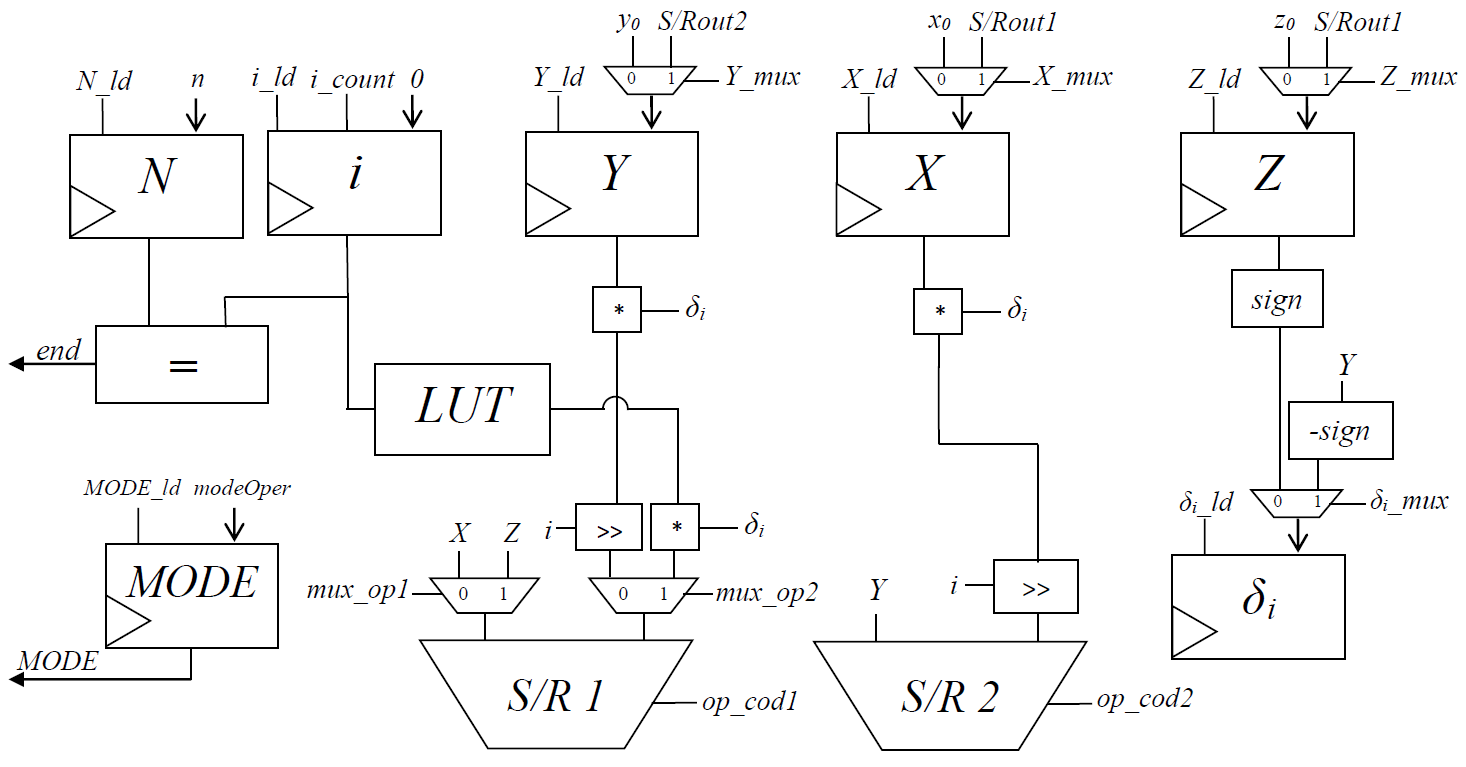
\includegraphics[scale=0.5]{images/Ruta de datos.png}
      \caption {Ruta de datos}
      \label{fig:RdD}
\end{figure}
\end{landscape}
\begin{landscape}
\setlength{\tabcolsep}{2pt}
\begin{figure}[h]
\begin{center}
    \begin{tabular}{ c| c|*{2}{c} |c|*{2}{c} |*{2}{c} |*{2}{c} |*{2}{c} |*{3}{c} |c }
        Estado & N\_ld&i\_ld&i\_count&MODE\_ld&Y\_ld&Y\_mux & X\_ld &X\_mux&Z\_ld&Z\_mux&\delta_i\_ld&\delta_i\_mux&mux\_op1&mux\_op2&op\_cod1&op\_cod2 \\ \hline
        S0 & 0&0&0&0&0&0&0&0&0&0&0&0&0&0&0&0 \\
        S1 & 1&1&0&1&1&0&1&0&1&0&0&0&0&0&0&0 \\
        S2 & 0&0&0&0&0&0&0&0&0&0&0&0&0&0&0&0 \\
        S3 & 0&0&0&0&0&0&0&0&0&0&1&0&0&0&0&0 \\
        S4 & 0&0&0&0&0&0&0&0&0&0&1&1&0&0&0&0 \\
        S5 & 0&0&0&0&0&0&0&0&1&1&0&0&1&1&$+$&0 \\
        S6 & 0&0&1&0&1&1&1&1&0&0&0&0&0&0&$-$&$+$ \\
    \end{tabular}
\end{center}
\caption {Tabla de señales de control}
      \label{fig:Tb}
\end{figure}

Nótese que en la ruta de datos aparece un módulo etiquetado como ``*'' que no es un multiplicador. Simplemente opera el signo del número introducido con $\delta_i$, lo que requerirá el uso de puertas lógicas y dependerá de la forma de representación elegida, pero nunca de un módulo multiplicador que es lo que pretendemos evitar a toda costa. De igual manera, los módulos ``sign'' y ``-sign'' calculan el signo y menos el signo de manera abstracta, huyendo de las implementaciones concretas. Por otro lado, en la tabla de señales de control tomamos el convenio de que, cuando nos es indiferente el valor que toma la señal, la ponemos a 0, y en el caso de los códigos de operación para los sumadores restadores, que nos dicen si se debe sumar o restar, indicamos la operación a realizar como $+$ o $-$ abstrayéndolo de cada codificación particular.
\end{landscape}

\printbibliography

\end{document}
